\section{TIES}

Relative alchemical free energy calculations were done between five pairs of the intercalator from the original experimental study. As discussed above, there are two groups of intercalator there: the four and five membered ring scaffolds. Pairs were selected based on two criteria: first to maximise the experimental free energy difference and second to sample all three possible combinations of transformation (between the 4 ring systems, 5 ring systems, and a transformation from 4 ring to 5 ring). 

As seen in figure~\ref{fig:ties} the correlation to experiment is poor. This can be for a number of reasons, but investigating more systems could be insightful. The experimental results for this study indicate binding affinities that are very close to each other, and even the best methods will struggle to differentiate between them. In the future we will collect and simulate intercalator ligand systems with experimental free energy differences large enough to be probed computationally. The simulations do converge as seen in figure~\ref{fig:ties_conv} well before the end of the simulation time. Still, TIES does produce more accurate results then the more approximate methods like ESMACS or docking. The root mean squared error on this small set of transformations is 0.41 kcal/mol.

\begin{figure}
  \centering
  \begin{tikzpicture}
\begin{axis}[
  ylabel=Predicted $\Delta \Delta G$,
  xlabel=Experimental $\Delta \Delta G$,
  ]
  
  \addplot[blue, mark=*, only marks] table {ties.csv};
  
\end{axis}  
\end{tikzpicture}
  \caption{Correlation plot comparing the experiment free energy difference with the calculated values via TIES. The experimental values are too close to each other, and the difference is smaller than the resolution of the TIES method given the 5 replicas used here. Furthermore the experimental error becomes large when we take the free energy difference between two values.}
  \label{fig:ties}
\end{figure}

\begin{figure}
  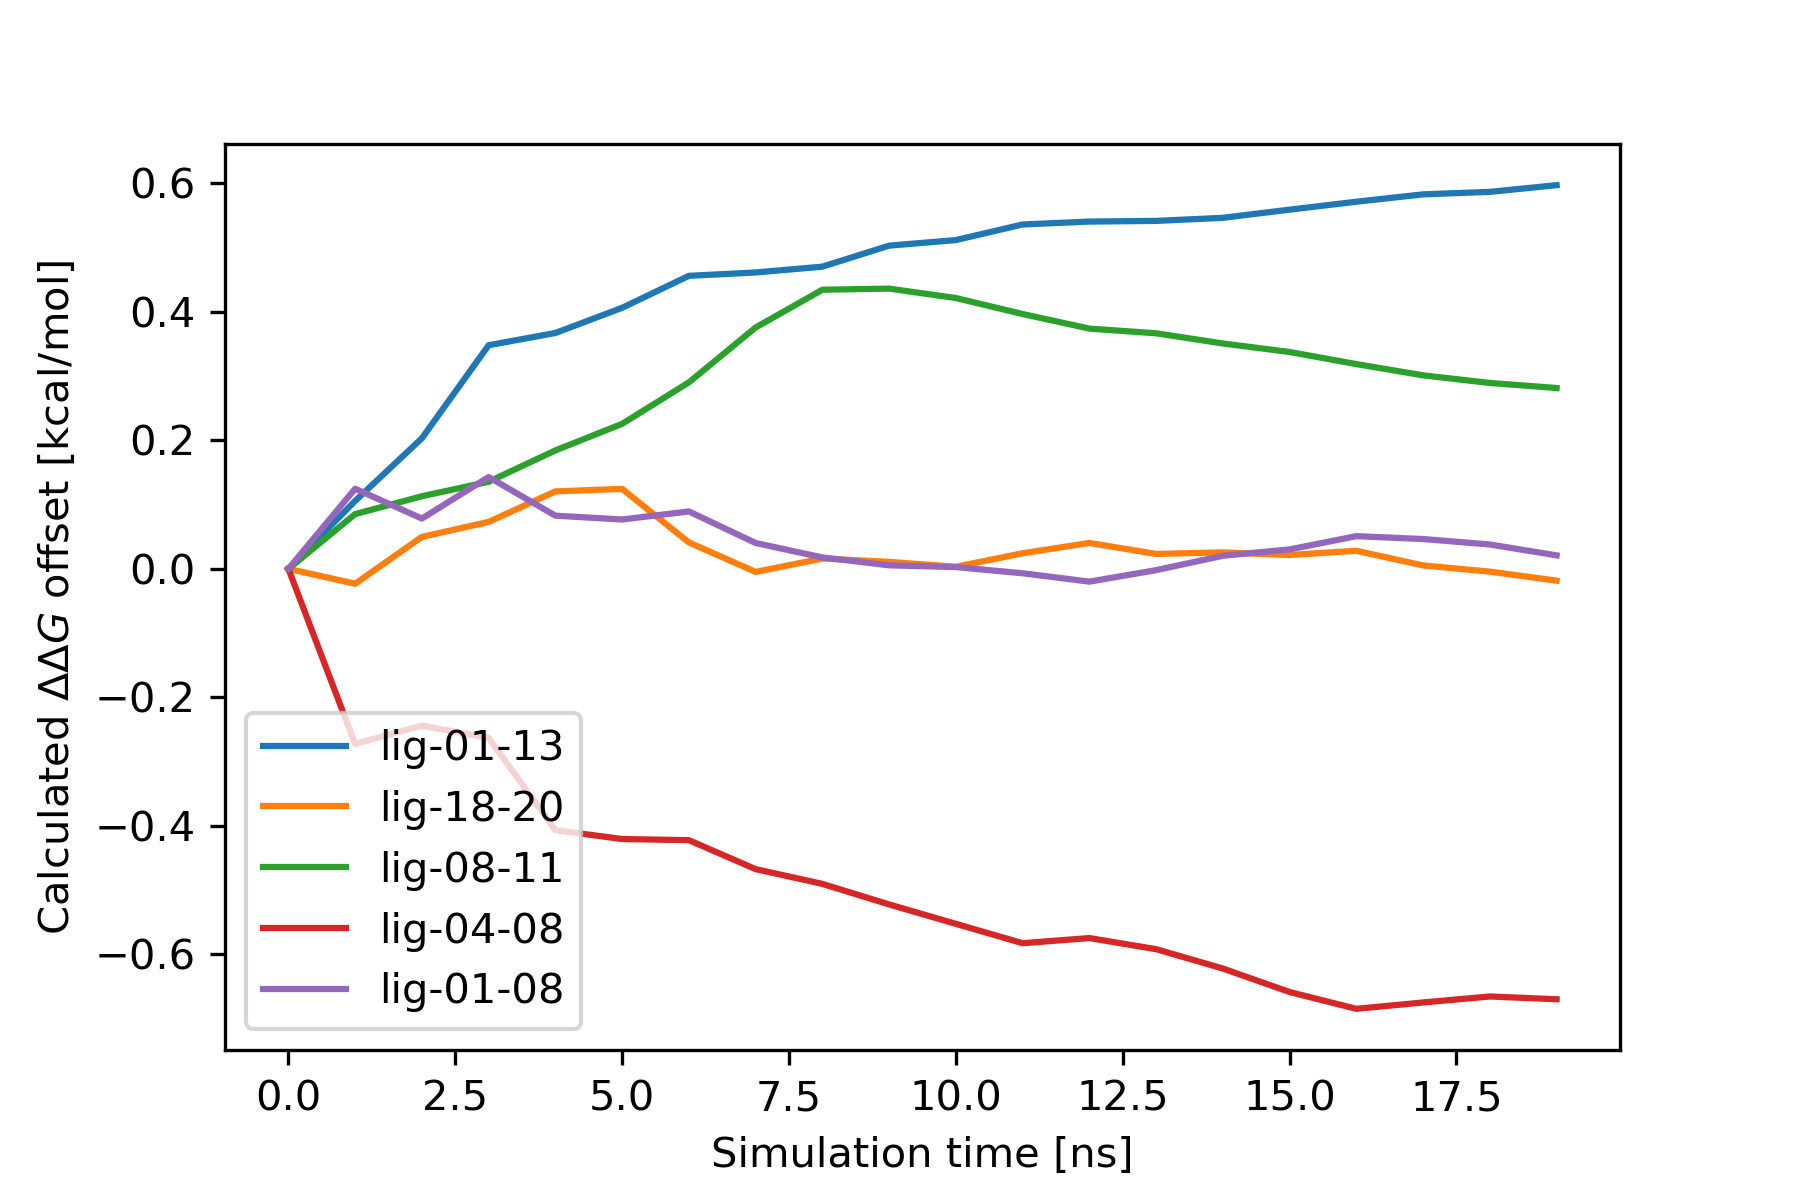
\includegraphics[width=\columnwidth]{ties_conv.png}
  \caption{Time evolution of the free energy difference for the five intercalator pairs investigated. The results are levelled off indicating that we reached converged values. The values are offset so they all start at point zero for illustrative purposes.}
  \label{fig:ties_conv}
\end{figure}